% Chapter 4 -- analysis, limitations, bonus scale discussion, conclusion.
\chapter{分析与讨论}\label{ch:analysis}

\section{停用词界线与文档粒度}

“线画在哪里”没有唯一正确的答案，它取决于语料、文档粒度和查询意图。本项目把线画在 $df\_ratio = 0.40$ 的候选带，再人工保留结构性功能词，得到 39 词表。这个选择有四点依据：

\begin{enumerate}
  \item \textbf{0.75 的粗筛线漏掉太多功能词。} 154 首十四行诗很短，很多对话中的功能词（如 \code{you}、\code{me}、\code{be}）在诗歌中不出现，$df\_ratio$ 被稀释。如果只看 0.75，只得到 9 个词，过滤后仍保留大量噪声。
  \item \textbf{0.40 之后开始混入内容词。} 在 0.40 档，新增词中出现了 \code{love}、\code{time}；它们虽然高频，但在文学检索中有实际意义，不应删除。把线停在 0.40，再用“结构性功能词”做人工判定，可以在“去噪”和“保留检索价值”之间取得平衡。
  \item \textbf{文档粒度会改变 df。} 本项目采用“一个完整作品 = 一个文档”（195 篇）。如果把 154 首十四行诗合并成 1 篇（42 篇文档），诗歌对 df 的稀释会减弱，候选表会整体上移。粒度敏感性实验留作后续工作；本文的 39 词表是针对当前 195 文档粒度推导的，不是普适常数。
  \item \textbf{熵规则把“人工审核”变成了可执行、可扫描的统计规则。} $df\_ratio \ge 0.40$ 且 $entropyRateNorm \ge 0.93$ 自动得到 39 词，与人工 39 词表重叠 35；差异恰好是 4 个古语功能词（自动版加入）和 4 个通用功能词（自动版漏掉），没有离群误报。这比“拍脑袋列一张表”更可复现，也更容易换语料重跑。
\end{enumerate}

另一个证据是 \code{the} 的 $df\_ratio$ 只有 90.8\%，而不是接近 100\%：154 首短诗中没有出现 \code{the} 的篇目不少。这说明 $df\_ratio$ 的绝对值高度依赖文档粒度；跨语料比较时更稳妥的指标是 $tf\_share$ 与词性/功能类别的结合。

\textbf{跨语料验证}：在 RFC 第二语料上，同一规则（0.40/0.001/0.93）推导出 \textbf{58 个词}，与莎士比亚的 9/39 个候选显著不同——这正是“没有万能停用词表”的直接证据。关键对照是 RFC 2119 的 \code{must / may / should}：它们 $df\_ratio = 1.0$（三篇全覆盖），但速率分布倾斜（RFC 7231 满篇 MUST，RFC 1035 很少用），$entropyRateNorm < 0.93$，因此没有被误判为停用词。旧的 df+tf 两特征规则会把它们连同 \code{server/mail/request} 一起收进 127 词候选带；“平”这个维度在跨语料场景真实起作用。

\section{Zipf 分布与 hapax}

语料呈现典型的 Zipf 分布（图~\ref{fig:zipf}）：

\begin{itemize}
  \item 词型 25,705 个，其中 hapax 9,753 个，占 \textbf{38.0\%} 的词型；
  \item 但 hapax 只占 \textbf{1.1\%} 的 token；
  \item top 10 词项覆盖了相当大比例的 token，\code{the} 一个词就占 3.28\%。
\end{itemize}

这对索引设计有两个含义：

\begin{enumerate}
  \item \textbf{词表被大量低频词占据。} 14,937 个词干中，近一半只出现一次；如果为每个词项分配固定大小的词典节点，内存会被“长尾”吃掉。字典结构的选择必须考虑这一点。
  \item \textbf{高频词与低频词的处理策略应不同。} 高频词（尤其是停用词）贡献了大部分 posting 长度和查询时的候选集，但区分度低；低频词区分度高，但 posting 很短。停用词过滤、\code{--max-df}/\code{--min-df}、\code{--top-x} 都是在这条长尾上做取舍。
\end{enumerate}

一个有趣的反作用：在正式配置中，最高频的词（\code{the/and/...}）已经被停用词表过滤掉，伸展树面对的 Zipf 偏斜被削弱了。这解释了为什么 splay 的比较次数（$\approx 11.5$ 次/访问）只比平衡树理论下界 $\log_2 14937 \approx 13.9$ 好一点，而没有出现“热点词全部贴近根”的极端优势。

熵特征从另一个角度补充了 Zipf 讨论：\textbf{词频的“量”与分布的“形状”是两件事}。\code{the} 的 tf 最高，但它的原始文档熵只有 0.724，因为长剧贡献了大部分出现次数；长度归一化后速率熵为 0.975，才恢复“按固定浓度撒在所有文档里”的直觉。$df$/$tf$ 只能判断“宽/重”，要判断“平”必须先把文档长度因素除掉。

\section{词典结构对比}

表~\ref{tab:dict-expanded} 把第 3 章的测量与结构性指标放在一起。

\begin{table}[H]
  \centering
  \caption{三种词典结构的综合对比}
  \label{tab:dict-expanded}
  \small
  \begin{tabularx}{\linewidth}{@{}l X X X@{}}
    \toprule
    指标 & 伸展树 & 哈希 & \code{std::map}（红黑树） \\
    \midrule
    构建耗时 & 0.35 s & \textbf{0.18 s} & 0.29 s \\
    字符串比较/访问 & $\approx 11.5$ & \textbf{$\approx 1.24$} & $\approx 14.5$ \\
    旋转 / rehash & 5,850,795 次旋转 & 11 次 rehash & 内部不可观测 \\
    有序输出 & 中序遍历，免费 & 收集后排序，$O(n\log n)$ & 中序遍历，免费 \\
    删除 & 不需要（只插不删） & 不需要 & 不需要 \\
    索引输出 & 逐字节一致 & 逐字节一致 & 逐字节一致 \\
    \bottomrule
  \end{tabularx}
\end{table}

哈希在纯构建速度与比较次数上明显胜出；伸展树的优势在于“冻结 term 表”时无需额外排序，且其自调整特性在热点明显的词流上更稳健。\code{std::map} 的比较次数最高（$\approx 14.5$/访问），但它的代价最稳定：严格 $O(\log n)$、没有旋转/重排副作用，且实现来自标准库。在本项目中，词表只有约 1.5 万项，三者都远未触及性能瓶颈；选择伸展树作为主结构更多是教学目的（对应课程对伸展树的要求）与结构性理由，而不是因为它在所有指标上更优。

哈希与 \code{std::map} 作为独立实现，最大的价值是提供了“三种实现产出同一索引文件”的交叉验证。如果把规模放大到百万级词表，哈希的 $O(1)$ 优势会更明显；但哈希无法支持前缀查询和有序遍历，需要额外的有序结构。“哈希构建 + 冻结有序表”的组合正是对讲义结论的呼应：哈希负责构建期的高速查找，冻结后的有序 term 表负责查询期的二分与前缀能力。

\section{索引压缩：v2 差分与变长编码}

当前 v1 格式直接存储 32 位整数：每个 posting 12 B（docID + tf + posStart），每个 position 4 B。正式索引 3,685,655 B 中，posting 与 positions 约 3.17 MB，term 表与头部约 0.5 MB。可压缩的空间主要来自：

\begin{enumerate}
  \item \textbf{docID 差分编码}：同一 term 的 posting 按 docID 递增，存储 gap 而不是绝对值；常见 gap 很小，可用变长字节编码。
  \item \textbf{positions 差分编码}：同一 posting 内 positions 递增，存储相邻位置差；短语查询仍然可以恢复绝对位置。
  \item \textbf{term 表前端编码（front coding）}：按字典序排列的 term 共享前缀，可只存“与上一个词的最长公共前缀长度 + 后缀”。
  \item \textbf{v2 版本字段}：索引头已有 \code{version}，v1 与 v2 只改变 postings 段编码，term 表/头部结构不变。
\end{enumerate}

\textbf{实现结果}：\code{mse build --compress} 写出 v2。postings 块按“docID gap、tf、position delta”的顺序编码，每个整数使用字节对齐变长码（首字节高 2 位给长度，低 6 位是低位；1--4 字节覆盖 6/14/22/30 位）。同一份正式索引的结果见表~\ref{tab:compression}。

\begin{table}[H]
  \centering
  \caption{索引压缩结果}
  \label{tab:compression}
  \small
  \begin{tabularx}{0.75\linewidth}{@{}l r r@{}}
    \toprule
    编码 & 索引字节 & 相对 v1 \\
    \midrule
    v1 原始 u32 & 3,685,655 & — \\
    v2 差分 + varint & \textbf{1,725,694} & \textbf{46.8\%} \\
    \bottomrule
  \end{tabularx}
\end{table}

构建耗时从 0.35 s 增至 0.48 s（编码开销）。正确性通过三条独立路径验证：\code{brute_force.py} 独立解析 v2 文件全词表对拍、\code{dump --verify-all} 对 14,937 词 0 差异、以及 varint 边界（6/14/22/30 位各档上下界加截断拒绝）单元测试。

为什么没有压到更小：term 表本身未压缩（约占 0.5 MB），每个 posting 的 tf 仍需编码，且高频词的位置差分仍有较大值。进一步的空间在 term 表前端编码、Elias $\gamma$/更紧凑的位级编码，以及按块选择编码方式；这些留作后续工作。压缩与磁盘词典 sidecar 正交：v2 索引可以配 B+Tree sidecar，两者可以叠加。

\section{查询阈值的语义与权衡}

阈值实验揭示了一个重要区别：\textbf{阈值作用于“查询词”，而不是直接作用于“结果文档”}。

\begin{itemize}
  \item \code{--max-df} 与 \code{--min-df} 是\textbf{词侧截断}：它们先决定“哪些查询词参与匹配”，再由匹配结果决定文档集。因此，单词查询被丢词后结果直接归零；多词 AND 查询被丢词后可能“放宽”为更少的词，结果反而变多（\code{sweet sword moon} 在 \code{--min-df 50} 下从 30 篇变为 90 篇）。
  \item \code{--min-match} 是\textbf{布尔语义的松紧}：它不丢弃词，只改变“至少命中几个词才算命中”。$k=1$ 即 OR，$k=\text{termCount}$ 即 AND。
  \item \code{--top-x} 是\textbf{结果侧截断}：它按得分保留前 $n$ 篇，不改变匹配语义，但会牺牲召回率。Jaccard 随 $x$ 单调回升，符合预期。
\end{itemize}

从系统设计角度看，索引期截断与查询期截断是两种不同的权衡（表~\ref{tab:truncation}）。

\begin{table}[H]
  \centering
  \caption{两种截断位置的权衡}
  \label{tab:truncation}
  \small
  \begin{tabularx}{\linewidth}{@{}l X X@{}}
    \toprule
    截断位置 & 优点 & 缺点 \\
    \midrule
    建索引期（讲义的 top-$x$ posting） & 索引体积小、查询快 & 一旦截断，后续查询无法恢复被丢弃的文档；构建成本高 \\
    查询期（本项目的 \code{--top-x}） & 保留完整索引，阈值可按查询调整，灵活 & 查询时需要遍历完整 posting，长 posting 的代价高 \\
    \bottomrule
  \end{tabularx}
\end{table}

本项目的选择是“查询期截断”，因为课程语料规模不大，保留完整索引更利于实验与对拍；如果面向大规模语料，则应考虑索引期截断、分层索引或 WAND 等提前终止算法。

另一个设计行为是短语查询不受词侧阈值影响。这是语义决定的：短语是一个整体，丢掉任何一个词都不再是原短语。第 3.8 节用 Jaccard 恒 1.00 验证了这一点。

\section{局限性与改进方向}

\subsection{已知局限}

\begin{enumerate}
  \item \textbf{短语在“过滤后 token 流”上匹配。} 这是本项目最重要的语义局限：\code{my lord} 会退化为 \code{lord}，\code{to be or not to be} 会因为全部是停用词而返回空集。讲义中提醒过这个例子；本项目选择“先滤后干”的管线，因此必须把这一点写入文档并配测试。
  \item \textbf{停用词查询返回空集。} 这是过滤索引的预期行为，但对用户来说可能不直观；系统用 note 行解释原因。
  \item \textbf{排序只使用 matched 与 $\Sigma tf$}，没有 TF-IDF、BM25、文档长度归一化等相关性模型；对于“返回文档 ID”的任务要求已经足够，但检索质量有提升空间。
  \item \textbf{文档粒度固定为作品级。} scene 级 manifest（约 1,080 篇）只预留为实验，尚未完成；粒度会显著影响 df 与停用词候选表。
  \item \textbf{只支持 ASCII。} 全语料非 ASCII 字符为 0，因此当前实现按字节处理；换语料（尤其是中文）需要重写分词与规范化。
  \item \textbf{默认构建仍是全内存。} B+Tree + SPIMI 已给出扩展路径，但 500,000 文件、400,000,000 词的真实构建没有跑过；当前实现可以在单机处理百万级词表/千万级 token。
  \item \textbf{B+Tree sidecar 由内存索引 bulk-load 生成。} 它解决了查询侧的词典常驻问题，但构建侧仍需要先有内存索引；完整的外部构建需要把 SPIMI 的 run 直接写成磁盘 term 表/B+Tree。
  \item \textbf{无并发、无增量更新。} 索引是只读快照，更新需要重建；分布式（按文档/按词切分）目前只有分析，没有实现。
  \item \textbf{plain 导入零清洗。} RFC 分页脚注 \code{[Page N]} 会原样入库，\code{page} 因此进入候选；清理属于 producer 职责（\code{extract.py} 对应莎士比亚，\code{import_corpus.py} 对应任意语料）。
\end{enumerate}

\subsection{改进方向}

\begin{itemize}
  \item 完成 scene 级粒度与“154 首合并”的敏感性实验；
  \item 增加排序模型（TF-IDF/BM25）并与 \code{--top-x} 结合；
  \item 把 SPIMI 的 run 直接写成磁盘 term 表/B+Tree，跑一次 500,000 文件级构建；
  \item term 表前端编码、Elias $\gamma$、块级自适应压缩；
  \item 分布式按文档/按词切分的原型与查询合并；
  \item 代码注释率已补齐：\code{src/} 与 \code{include/} 的非空行注释率约 31\%，高于课程 30\% 的硬性要求。
\end{itemize}

\section{Bonus：500,000 个文件与 400,000,000 个不同单词}

\subsection{结论先行}

\textbf{当前的全内存实现不能直接处理这个规模。} 400M 个不同词、500k 个文件意味着：

\begin{itemize}
  \item 词典项 400M：按每项 100--150 B（字符串 + 节点 + 元数据）估算就是 40--60 GB；
  \item 若按当前语料外推（每篇约 4,444 token，posting/token $\approx 0.211$），500k 篇约 22 亿 token、4.7 亿条 posting、22 亿个 position；posting 5.6 GB + position 8.9 GB；
  \item 语料文本本身约 12.5 GB（按平均 25 KB/篇估算）；
  \item 合计约 70--90 GB，尚未计 vector 容量冗余、哈希桶、构建期临时结构。
\end{itemize}

普通工作站（16--64 GB）无法容纳，单机全内存构建的时间和内存压力也不可接受。另一个边界是 32 位字段：当前 \code{posStart} 是 u32，总 token 超过 $2^{32} \approx 42.9$ 亿时会溢出；本估算的 22 亿尚未越界，但更大规模应改 u64。

针对这个问题，本项目实现了三块可实测的组件：构建侧的 SPIMI 块式外部构建、查询侧的磁盘 B+Tree 词典、以及 v2 posting 压缩；并用 RFC 第二语料验证语料无关性。此外，500,000 文件 / 20,000,000 token 的合成语料已实际跑批（4.7.2 节），B+Tree 已实测到 50,000,000 键（4.7.5 节）。

\subsection{构建侧：SPIMI 块式外部构建}

\code{mse build-blocks --block-terms N} 按文档流扫描，块内词典达到 $N$ 个 term 就排序落盘成 run 文件，最后按词 $k$ 路归并。内存上界是 $O(N)$，与语料总词表无关；块边界只切在文档边界，因此同一词在后续 run 中的 docID 一定更大，归并时直接拼接 postings。

正式配置（budget 4096）的实测见表~\ref{tab:spimi-formal}。

\begin{table}[H]
  \centering
  \caption{SPIMI 块式构建（正式语料）}
  \label{tab:spimi-formal}
  \small
  \begin{tabularx}{0.72\linewidth}{@{}X r@{}}
    \toprule
    指标 & 数值 \\
    \midrule
    run 数 & 17 \\
    峰值活词 & 5,129（预算 + 单文档新增的合理超出） \\
    临时 run 字节 & 4,166,556 B \\
    扫描时间 & 0.36 s \\
    归并时间 & 0.06 s \\
    产物 & 与 \code{mse build} 逐字节一致 \\
    \bottomrule
  \end{tabularx}
\end{table}

这说明构建侧的内存可以被块预算控制住。为了验证“500k 文件”这一侧，合成语料生成器构造了一套 plain 语料：500,000 个文档、每篇 40 token、词表上限 5,000,000。块式构建（预算 50000）的实测见表~\ref{tab:spimi-500k}，生成命令见附录~\ref{app:build}。

\begin{table}[H]
  \centering
  \caption{500k 文件合成语料的块式构建}
  \label{tab:spimi-500k}
  \small
  \begin{tabularx}{0.85\linewidth}{@{}X r@{}}
    \toprule
    指标 & 数值 \\
    \midrule
    文档 / token & 500,000 / 20,000,000 \\
    不同词 & 4,908,747 \\
    run 数 / 峰值活词 & 398 / 50,039 \\
    临时 run 字节 & 558,397,200 B \\
    扫描 / 归并 & 9.98 s / 30.00 s \\
    峰值内存 & 1.50 GB \\
    索引 & 427,603,247 B \\
    对照 & 与内存 \code{mse build} 逐字节一致（内存构建 65.9 s / 2.43 GB） \\
    \bottomrule
  \end{tabularx}
\end{table}

500k 文件侧已经实际跑通；词表是 \textbf{4.9M} 而不是 400M（生成 400M 个不同词需要数百 GB，见 4.7.1 节）。400M 词侧的查询证据由 4.7.5 节的 \textbf{50M 键 B+Tree 实测}与线性外推给出；构建侧若继续放大，run 数会随词表/预算增长，需要在多趟归并、磁盘吞吐和临时空间之间做工程权衡（讲义对 4 亿条三元组、40 MB 内存的估算是约 100 个 run、7 趟归并、约 20 小时、临时空间约文本的 2 倍）。

\subsection{查询侧：磁盘 B+Tree 词典}

\code{mse build --dict-file} 把 term 到 (posting offset, length) 的映射冻结成页式 B+Tree sidecar。查询时只加载文档表，term 经 B+Tree 的 $O(\text{height})$ 页读定位，再 seek 到 posting 字节；词表与 postings 不整体加载。

正式索引（14,937 词）的实测见表~\ref{tab:bptree-formal}。

\begin{table}[H]
  \centering
  \caption{磁盘 B+Tree 词典（正式索引）}
  \label{tab:bptree-formal}
  \small
  \begin{tabularx}{0.85\linewidth}{@{}X r@{}}
    \toprule
    指标 & 数值 \\
    \midrule
    sidecar 大小 & 237,568 B（58 页 $\times$ 4 KiB，高 2），占索引 6.4\% \\
    冷查询 \code{banquo} & 词典 2 页 + 索引 8,308 B $\approx$ 16.5 KB \\
    相对全量加载 & 0.45\% \\
    全词表 \code{--verify-all} & 14,937 词 0 差异；114 次页读 + 29,819 次缓存命中 \\
    查询输出 & 与全量加载文本/JSON 逐字节一致 \\
    \bottomrule
  \end{tabularx}
\end{table}

B+Tree 的设计要点：页预算与序列化布局严格对应；变长键下分裂取“合法窗口内的字节中点”，并用可证下界 $\text{pageSize}/2 - \text{maxEntry}$ 作为填充不变量；分隔键是真实键的副本，因此内部路由区间左闭。\code{tests/test_bptree.cpp} 用 \code{std::map} oracle 覆盖三档页宽、对抗性同前缀键、bulk-load 与逐条插入等价、文件往返、坏魔数拒绝等 10 个用例、84,648 条断言。

\subsection{压缩：v2 差分与变长编码}

v2 把 postings 改为“docID gap、tf、position delta”，每个整数使用字节对齐变长码；头部/文档表/词表布局与 v1 相同，靠版本字段区分。正式索引从 3,685,655 B 降到 1,725,694 B（46.8\%），构建时间从 0.35 s 增至 0.48 s。正确性方面，\code{brute_force.py}、\code{dump --verify-all} 和 varint 边界测试全部通过。压缩与 B+Tree sidecar 正交，可以叠加使用。

\subsection{规模实测与外推}

\code{mse bptree-bench --keys N} 用递增 base-26 合成键 bulk-load 落盘，再用缓存 = 1 页的读取端做随机查询，结果见表~\ref{tab:bptree-scale} 与图~\ref{fig:bptree}。

\begin{table}[H]
  \centering
  \caption{B+Tree 规模实测}
  \label{tab:bptree-scale}
  \small
  \begin{tabularx}{\linewidth}{@{}r r r r r r@{}}
    \toprule
    键数 & 树高 & 页数 & 文件大小 & 字节/键 & 每次查询页读 \\
    \midrule
    100,000 & 2 & 369 & 1,515,520 B & 15.16 & 2.00 \\
    1,000,000 & 3 & 3,688 & 15,110,144 B & 15.11 & 3.00 \\
    10,000,000 & 3 & 36,865 & 151,003,136 B & 15.10 & 3.00 \\
    30,000,000 & 3 & 110,593 & 452,993,024 B & 15.10 & 3.00 \\
    50,000,000 & 4 & 184,322 & 754,987,008 B & 15.10 & 4.00 \\
    \bottomrule
  \end{tabularx}
\end{table}

\begin{figure}[H]
  \centering
  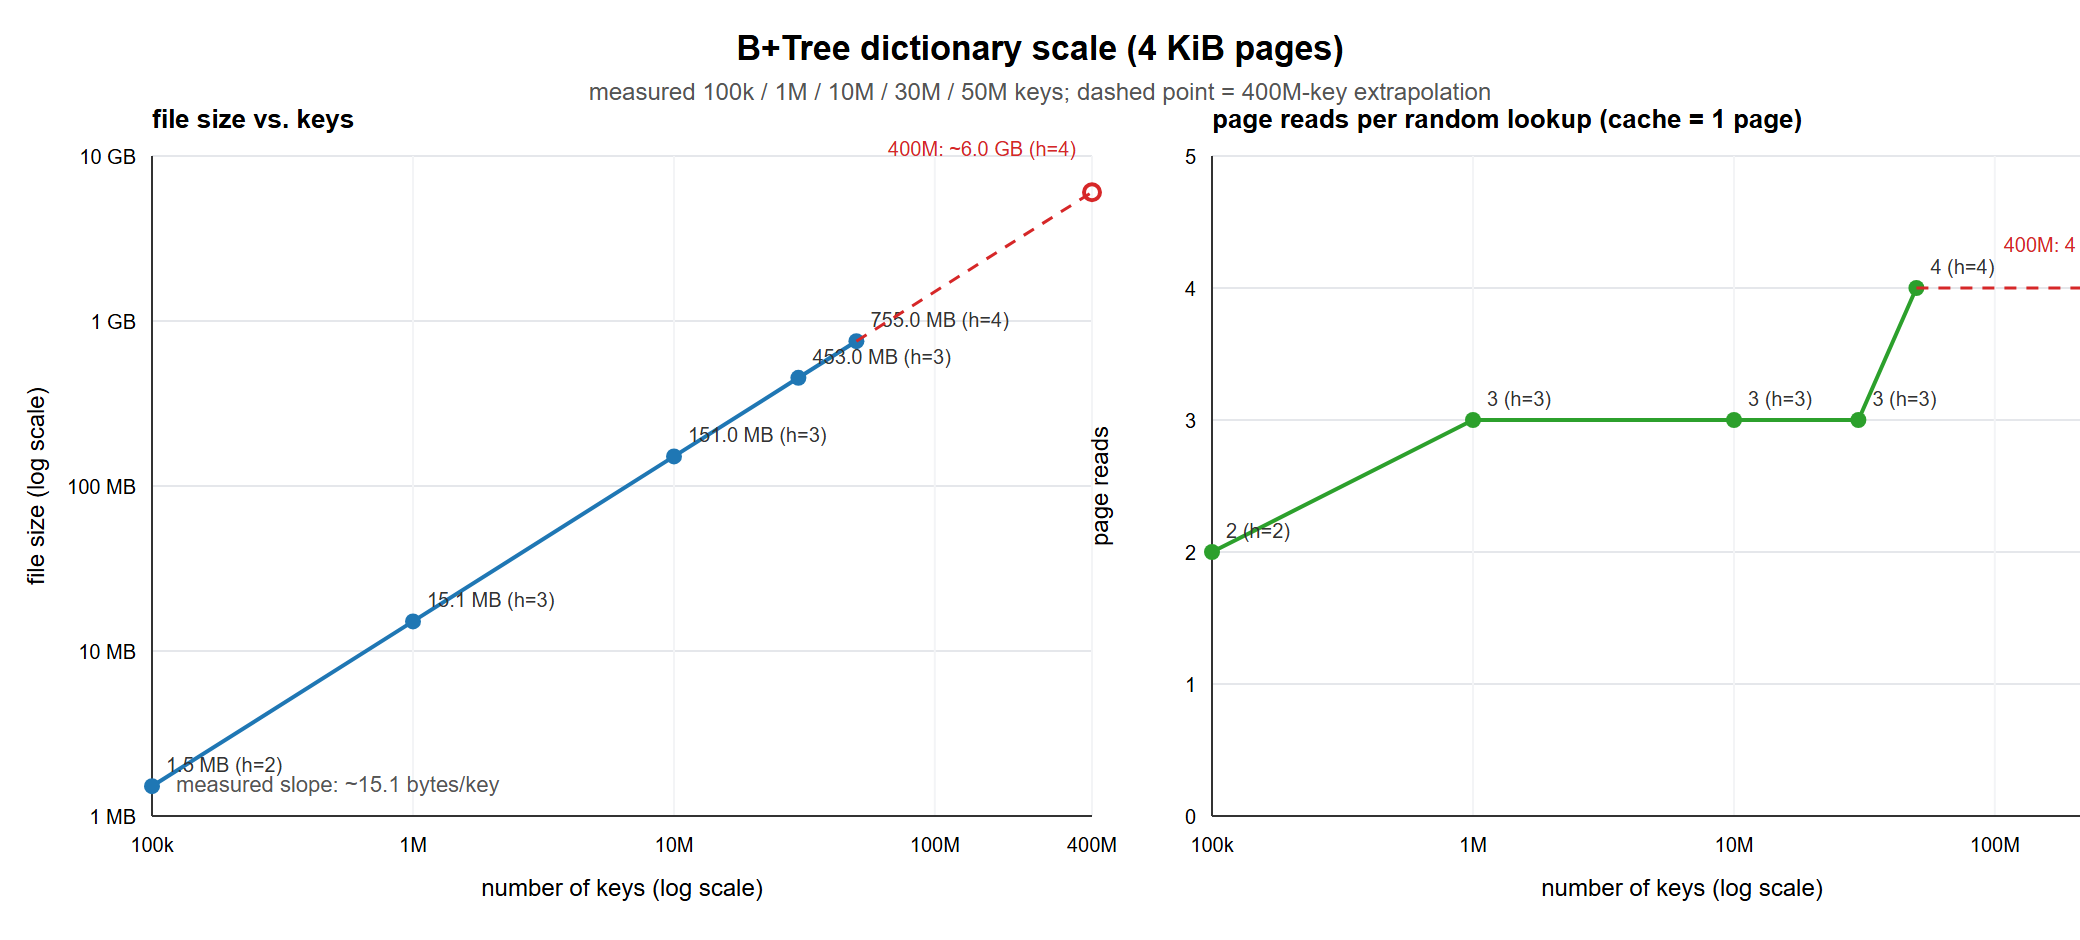
\includegraphics[width=0.92\linewidth]{figures/bptree_scale.png}
  \caption{B+Tree 的规模实测。左图为文件大小（双对数），右图为每次随机查询的页读；100k/1M/10M/30M/50M 为实测点，400M 为按 15.1 B/键与扇出公式的外推点。}
  \label{fig:bptree}
\end{figure}

体积严格线性（约 15.1 B/键），高度与扇出计算吻合。\textbf{50M 键实测已经进入 height 4、每次查询 4 页}，与 400M 外推处于同一高度档；按同一公式外推：

\begin{itemize}
  \item 100M 键 $\approx$ 1.5 GB，树高 4；
  \item 400M 键 $\approx$ 6.0 GB（键长可能略增，取 6--6.5 GB），树高 4；
  \item 单次查询 4 页 $\approx$ 16 KB。
\end{itemize}

也就是说，\textbf{词典无法常驻内存时，查询仍然只付 4 次页读的代价}。构建侧需要把 400M 个 term 写入这个 B+Tree（bulk-load 要求输入已排序；可以由 SPIMI 的归并输出提供），这是下一步的工程工作。

\subsection{语料无关性验证：RFC 第二语料}

\code{data2/} 收录 RFC 1035/5321/7231 三篇 plain 文本（3 文档、9,946 行、75,250 token、4,328 词型）。用同一套 C++ 管线跑通：

\begin{itemize}
  \item \code{stats / count / stopwords --derive / build / query / brute_force} 零代码改动；
  \item count CSV 与 Python 对拍逐字节一致；
  \item 熵规则推导出 58 词（与莎士比亚的 9/39 不同），\code{must / may / should} 因速率分布倾斜未被判为停用词；
  \item 建索引 2,660 词干 / 4,594 postings / 45,370 token / 308,164 B，brute-force 全项一致；
  \item \code{smtp}、\code{domain} 各命中 3 篇；\code{server} 被判为停用词，返回空加 note。
\end{itemize}

这组实验说明：引擎本身不依赖莎士比亚；换语料只需要 producer 提供 manifest 与文本层，停用词可以由规则重新推导。

\subsection{仍然存在的边界}

\begin{enumerate}
  \item \textbf{500k 文件已跑通，400M 词没有真正生成}：500k 文件 / 20M token / 4.9M 词的合成跑批已完成（4.7.2 节）；400M 个不同词需要数百 GB，当前用 50M 键 B+Tree 实测加线性外推（4.7.5 节）给出查询侧证据。
  \item \textbf{B+Tree 由内存索引 bulk-load}：查询侧已去掉常驻词典，构建侧仍需要先把索引放在内存；完整方案应让 SPIMI 归并直接产出 B+Tree 页文件。
  \item \textbf{分布式未实现}：按文档切分（构建均衡、查询广播）与按词切分（查询局部、热点词）的权衡只有分析；GFS 式的块复制/容错也没有落地。
  \item \textbf{32 位字段}：\code{posStart}/\code{tf} 在更大规模下应改 u64；\code{docID} 的 u32 对 500k 文件足够。
  \item \textbf{磁盘/内存成本}：400M 词的 B+Tree 约 6 GB，SPIMI 临时空间约为语料的 2 倍；这些是实际部署必须预算的。
\end{enumerate}

\textbf{结论}：全内存版本不能直接工作；但“SPIMI 构建 + B+Tree 词典 + v2 压缩”的组合已经把构建侧和查询侧的关键瓶颈分别解决到可实测、可外推的程度。距离完整 500k/400M 跑批还差工程集成与分布式，而不是算法上的未知。

\section{结论}

本项目完成了题目要求的四项任务：在莎士比亚全集上实现了词频统计与停用词推导、带 Porter 词干化的倒排索引、单词/短语/布尔查询，以及四个查询阈值的系统性实验。正确性通过单元测试、黄金样例、独立 Python 对拍与全量 brute-force 四层验证；正式索引为 14,937 个词干、117,704 条 posting、556,866 个位置、v1 约 3.5 MB / v2 约 1.7 MB。Bonus 进一步实现了熵驱动停用词、RFC 第二语料、SPIMI 块式构建、磁盘 B+Tree 词典、500k 文件跑批与 5000 万键规模实测。

项目的主要经验是：

\begin{enumerate}
  \item \textbf{规格必须唯一且可执行}。分词、标记行判定、停用词顺序、词干化变体，任何一处模糊都会在 C++ 与 Python 对拍中放大成数字差异。
  \item \textbf{独立实现的对拍比“再跑一遍”更有价值}。\code{brute_force.py} 从原始文本重建 posting，抓出了多个真实 bug；v2、B+Tree、SPIMI 的对拍也各抓出了实现问题。
  \item \textbf{阈值作用于查询词，而不是结果}。这是理解 \code{--max-df}/\code{--min-df} 行为的关键，也是多词查询可能出现“丢词反而结果变多”的原因。
  \item \textbf{“去噪”可以用统计规则表达}。长度归一化速率熵把“停用词按固定浓度撒在文档里”这一直觉变成可执行规则；换语料后阈值仍需重新扫描，但方法不再依赖人工列表。
  \item \textbf{全内存设计的边界清晰，扩展路径也已实测}。SPIMI 控制构建内存、B+Tree 控制查询侧词典内存、v2 控制索引体积；距离完整的 500k/400M 跑批还差工程集成与分布式，而不是算法上的未知。
\end{enumerate}

后续工作包括：完成 scene 级/154 首合并的粒度敏感性实验；把 SPIMI 的 run 直接写成磁盘 term 表/B+Tree 并跑一次 500k 文件级构建；补 term 表前端编码与更紧凑的位级压缩；完成分布式原型。
